\documentclass[11pt]{article} 
\usepackage{stmaryrd, amsfonts, amsmath, pifont, fullpage, natbib, color, setspace, graphicx, linguex, multirow}
\definecolor{darkblue}{rgb}{0.2,0.2,0.7}
\author{ {\it Submitted to Australasian Journal of Philosophy for anonymous review}
 }
\date{}   
\title{New horizons for a theory of epistemic modals}

%New Symbols
\DeclareSymbolFont{symbolsC}{U}{txsyc}{m}{n}
\DeclareMathSymbol{\strictif}{\mathrel}{symbolsC}{74}
\DeclareMathSymbol{\boxright}{\mathrel}{symbolsC}{128}
\DeclareMathSymbol{\Diamondright}{\mathrel}{symbolsC}{132}
\DeclareMathSymbol{\Diamonddotright}{\mathrel}{symbolsC}{134}
\DeclareMathSymbol{\Diamonddot}{\mathord}{symbolsC}{144}
\newcommand{\xmark}{\ding{55}}

 %TC:newcounter fwords Words in footnotes
    %          TC:newcounter footnote Number of footnotes
       %       TC:macro \footnote [fwords]
          %    TC:macroword \footnote [footnote]			

%New commands
\newcommand{\bitem}{\begin{itemize}}
\newcommand{\eitem}{\end{itemize}}
\newcommand{\lang}{$\langle$}
\newcommand{\rang}{$\rangle$}
\newcommand{\back}{$\setminus$}
\newcommand{\HRule}{\rule{\linewidth}{0.1mm}}
\newcommand{\llm}[2][]{$\llbracket${#2}$\rrbracket^{#1}$}
\newcommand{\ul}{$\ulcorner$}
\newcommand{\ur}{$\urcorner\ $}
\newcommand{\urn}{$\urcorner$}	

\begin{document}

\maketitle

\begin{abstract}\noindent Recent debate over the semantics and pragmatics of epistemic modals has focused on intuitions about cross-contextual truth-value assessments. In this paper, we advocate for a different approach to evaluating theories of epistemic modals. Our strategy focuses on judgments of the incompatibility of two different epistemic possibility claims, or two different truth value assessments of a single epistemic possibility claim. We subject the predictions of existing theories to empirical scrutiny, and argue that existing contextualist and relativist theories are unable to account for the full pattern of observed judgments. As a way of illustrating the theoretical upshot of these results, we conclude by developing a novel theory of epistemic modals that is able to predict the results. \begin{center} {\bf Keywords}: epistemic modals, contextualism, relativism, truth.\\ {\bf Word count}: 7,924 \end{center}\end{abstract}

\begin{doublespace}

\noindent At the core of the recent debate over the semantics of modals is a tension between modal language and its subject matter. Consider the following modal sentence:

\ex. The keys might be in the drawer.\label{keys}

On the epistemic interpretation of ``might,'' this sentence seems to state that it is epistemically possible that the keys are in the drawer. However, it also seems that there are no such absolute epistemic possibility facts: rather, propositions are only epistemically possible relative to a body of evidence or information. Suppose Jones doesn't know whether the keys are in the drawer, but Smith has seen that they aren't. Then, relative to Jones' evidence, it is epistemically possible that the keys are in the drawer, but relative to Smith's evidence, it is \textit{not} epistemically possible that the keys are in the drawer. Thus, we face a mismatch between the subject matter of epistemic modality and the language we use to talk about it: propositions are only epistemically possible relative to a body of evidence, but such relativization is not explicitly marked in  sentences like \ref{keys}.%\footnote{Not all epistemic modal claims are absolutist. Some make explicit the relevant relativization:

%\ex. According to John, the keys might be in the drawer.

%Our point above is just that sentences like \ref{keys} lack this kind of overt relativization.}

Existing semantic theories of epistemic modals resolve this tension in different ways. For instance, modal contextualism proposes that epistemic modal sentences like \ref{keys} do in fact express propositions about particular bodies of evidence. Contextualism holds that {\it which} body of evidence a particular epistemic modal claim is about depends on the context in which it is uttered (\citealt{hacking:1967, kratzer:1981, kratzer:1991, derose:1991, stanley:2005b, dowell:2011}). 

By contrast, modal relativism resolves the tension by proposing that epistemic modal sentences express propositions that are not about particular bodies of evidence, but are instead true or false relative to bodies of evidence (cf. \citealt{egan:2005, egan:2007, macfarlane:2011a, macfarlane:2014a}). An important commitment of relativism is that the same epistemic modal proposition may be true as assessed in one context and false as assessed in another. 

The debate between modal contextualism and relativism has focused on cross-contextual assessments of speech acts involving bare epistemic modal sentences like \ref{keys}. These are cases where a better-informed eavesdropper evaluates the truth value of an epistemic modal claim made by a lesser-informed speaker in a different context. Our aim in this paper is to shift the perspective on this debate and advocate a different way of evaluating contextualist and relativist theories of epistemic modals. In $\S$\ref{1}, we argue for testing the predictions of contextualism and relativism by exploring intuitions about the (in)compatibility of epistemic modal claims across contexts. In $\S$\ref{2}, we report the results of a new empirical study, which reveals new data that neither existing contextualist nor relativist theories predict. This motivates the search for an alternative to orthodox contextualist and relativist theories; we sketch one such theory in $\S$\ref{3}. We conclude by considering how our approach may generalize to a broader range of linguistic expressions.

\section{Distinguishing Contextualism and Relativism}
\label{1}

Throughout, we focus on epistemic possibility sentences like \ref{keys}. We make the standard assumption that such sentences are composed of a modal, `might,' scoping over a sentence p. We use ` \ul might p\ur ' to denote the sentence schema whose substitution instances are epistemic possibility sentences like \ref{keys}; in such a sentence, ``might'' is the modal and p is its prejacent. Lowercase italic letters $p, q, r, \dots$ are used as variables over propositions. Finally, we assume that the truth of such sentences depends both on a modal base $f$ (a function from a world to a set of worlds; cf. \citealt{kratzer:1981}), and a world $w$, as follows:

\ex.[] {\sc Simple Semantics}\\
	{\ul might p\ur is true at $f,w$ iff $\exists w'\in f(w)$: p is true at $f,w'$.} 

Think of an epistemic modal base as a characterization of a body of information or evidence: what Jones knows, the information compatible with the security camera footage, and so on. Thus, we can read {\sc Simple Semantics} as stating that \ul might p\ur is true relative to a world and body of information iff p is compatible with that body of information (at that world). Contextualist and relativist theories differ as to how modal bases enter into the semantics and pragmatics of epistemic modals. 

Orthodox contextualist theories of epistemic modals are distinguished by two main claims:

\begin{itemize}
\item[(C1)] {\bf Context-dependence}: Epistemic modal sentences are context dependent; in different contexts, the same epistemic modal sentence may express different propositions.
\item[(C2)] {\bf Truth absolutism}: The proposition expressed by an epistemic modal sentence has its truth value fixed by the world. In other words, it determines a set of possible worlds.
\end{itemize}

\noindent Thus, contextualist theories hold that an epistemic modal sentence expresses a proposition that is about a particular modal base, which is determined by the context in which it is uttered. For instance, in context $c_1$, the sentence \ul might p\ur says that $p$ is compatible with evidence $f_{c_1}$ (i.e., it expresses the proposition $\lozenge_{c_1} p$); in context $c_2$, it says that $p$ is compatible with evidence $f_{c_2}$ (i.e., it expresses the proposition $\lozenge_{c_2} p$); and so on. 

By contrast, standard relativist theories of epistemic modals deny both (C1) and (C2), and instead endorse:

\begin{itemize}
\item[(R1)] {\bf Context-invariance}: Epistemic modal sentences are context invariant; in different contexts, the same epistemic modal sentence expresses the same proposition (so long as its prejacent is not context-dependent).
\item[(R2)] {\bf Truth relativism}: The truth value of the proposition expressed by an epistemic modal sentence can vary across dimensions of evaluation at the same world. 
\end{itemize}

\noindent Thus, according to the relativist, in every context, \ul might p\ur says that $p$ is epistemically possible. In other words, \ul might p\ur expresses the proposition $\lozenge p$, which is true relative to evidence $f$ iff $p$ is compatible with evidence $f$.\footnote{Formally, this difference amounts to a difference in the formal object the theories use to model the propositions expressed by epistemic modal sentences. For contextualists, the proposition expressed by \ul might p\ur at $c$ just is an ordinary possible-worlds proposition: $\{w: \exists w'\in f_c(w)$: p is true at $f,w'\}$. But for relativists, the proposition expressed by \ul might p\ur (in any context) is not reducible to a possible-worlds proposition. Instead, it is modellable as a world/evidence-proposition: $\{\langle w, f\rangle: \exists w'\in f(w)$: p is true at $f,w'\}$.}

The differences between these theories matter when it comes to norms governing the acceptance of propositions. Because of their commitment to (C2), contextualists can appeal to a norm involving  involving truth, knowledge, or justified belief that is not relativized to contexts. Here is one possible such norm:\footnote{We will focus on truth norms here, but this is just for the sake of concreteness. We do not want to take a stand on whether instead knowledge or justified belief or high credence of truth should be the norm of acceptance.}

\ex.[]  {\sc Truth Norm}\\
	{Accept $p$ only if $p$ is true.}
	%\b. Reject an assertion of proposition $p$ if $p$ is false.

However, the relativist's norm of acceptance makes important use of her commitment to epistemic modal propositions varying in truth value across contexts of assessment:

\ex.[] {\sc Relativist Truth Norm} \\
	{Accept $p$ at $c$ only if $p$ is true at $c$.}
	%\b. Reject (at $c_A$) an assertion of proposition $p$ made at $c_U$ if $p$ is false at $c_A$.

{\sc Relativist Truth Norm} entails that whether person A ought to accept $\lozenge p$ depends on whether the evidence in A's context is compatible with $p$. By contrast, {\sc Truth Norm} only applies to propositions whose truth value is fixed by the world: it says that whether A ought to accept $\lozenge_c p$ depends on whether $\lozenge_c p$ is true---that is, on whether the evidence in $c$ is compatible with $p$. Say that an orthodox contextualist theory is one that endorses (C1), (C2), and {\sc Truth Norm} and that an orthodox relativist is one that endorses (R1), (R2), and {\sc Relativist Truth Norm}. Thus understood, orthodox contextualist and relativist theories make different predictions about assessments of epistemic modal claims across contexts.
%\footnote{We can also distinguish both (standard) contextualism and relativism from non-indexical contextualism (\citealt{macfarlane:2009, macfarlane:2014a}). Non-indexical contextualism is the view committed to (R1) + (R2) + {\sc Contextualist Truth Norm}:

%\ex.[] {\sc Contextualist Truth Norm} \\
%	{Accept (at $c_A$) an assertion of proposition $p$ made at $c_U$ only if $p$ is true at $c_U$.}
	%\b. Reject (at $c_A$) an assertion of proposition $p$ made at $c_U$ if $p$ is false at $c_U$.

%} 

Before we get to the cases which have been used to distinguish contextualism and relativism, we articulate two more standard background assumptions that are necessary for generating predictions in such cases. The first is:

\ex.[] {\sc Says-Talk}\\
	{\ul X's claim\ur and \ul What X said\ur refer to the content of X's assertion on some particular occasion of utterance.}

This is a very orthodox assumption, shared by many contextualists and relativists, that goes back to \cite{kaplan:1989}. One motivation for this hypothesis is the behavior of indexicals in discourses like:

\ex. \a.[A:] I am hungry.
	\b.[B:] What A said is true.

Here, A utters the sentence, ``I am hungry'' and thereby asserts that A is hungry. What does B assert? Intuitively, B asserts something equivalent to: A is hungry. This is predicted by {\sc Says-Talk}: according to it, B refers to the proposition A asserted and asserts of it that it is true---as such, B asserts that the proposition that A is hungry is true, and this seems equivalent to asserting that A is hungry. 

The second assumption is a deflationary semantics for ``is true'' and ``is false'':

\ex.[] {\sc Deflationism} \\
	{The proposition expressed by \ul What X said is true\ur (\ul What X said is false\urn) is equivalent to the proposition (the negation of the proposition) referred to by \ul What X said\ur on that occasion of use.}
	
This principle is also widely accepted by both contextualists and relativists. We appealed to {\sc Deflationism} in generating the prediction that B says something equivalent to what A said. Furthermore, this principle does seem intuitively plausible: endorsing what someone says by calling it ``true'' does not seem to add anything to what they said. We return to both of these assumptions in more detail below.
	
\subsection{Eavesdropper Intuitions}
\label{1.1}

Given these assumptions, we can use intuitions about cross-contextual eavesdropper cases to test the predictions of orthodox contextualism and relativism. The reason to focus on cross-contextual eavesdropping is that in such cases the {\sc Truth Norm} and {\sc Relativist Truth Norm} can come apart, since the assessment takes place in a context that is distinct from the context in which the claim is made. Suppose A utters, \ul might p\ur and that B is not part of A's context, but is instead secretly listening in on A's conversation (perhaps via a wire tap). Given {\sc Says-Talk} and {\sc Deflationism}, contextualism predicts that whether B ought to think that what A said is true depends on whether the evidence relevant in A's context is compatible with $p$. By contrast, relativism  predicts that whether B ought to think that what A said is true depends on whether the evidence relevant in B's context is compatible with $p$. 

A common intuition alleged in the literature is that it would be correct for B to think that what A said is false, if B has evidence ruling out $p$, even if A's evidence was compatible with $p$ (cf. \citealt{egan:2005, egan:2007, macfarlane:2011a, macfarlane:2014a}). This intuition is easily explained by relativism, since according to relativism, it is B's evidence that matters to whether it would be correct for B to think that what A said is true. However, this intuition is not easily explained by contextualism, since according to contextualism, it is A's evidence that matters to whether it would be correct for B to think that what A said is true.%\footnote{This is not to say that it is {\it impossible} for a contextualist theory to predict this result, but that doing so would require building the eavesdropper's evidence into the evidence determined by the original speaker's context of utterance, and this may be implausible in many cases. One looming challenge (pressed aptly by \cite{macfarlane:2011}) is that building the eavesdropper's evidence into the evidence determined by the speaker's context risks making the truth value of many epistemic possibility sentences implausibly unknowable, and thus predicts that such sentences should be less easily assertable than they otherwise seem.}

Recently, however, this argument in favor of relativism over contextualism has been contested on the grounds that this intuition is not widely shared (see \citealt{dowell:2011, yalcinknobe:2014}). In what follows, we discuss the results of Knobe and Yalcin, who empirically tested intuitions in such a case. In their first study, they asked native English speakers to read a vignette about two Experts who viewed skillfully faked evidence that suggested that a mobster named Fat Tony was murdered at the docks. After viewing the evidence, Expert A makes a non-modal claim: ``Fat Tony is dead.'' Expert B instead makes a modal claim: ``Fat Tony might be dead.'' Participants were asked to rate their agreement with one of the following statements: 

\begin{itemize}
\item (nonmodal-true) What Expert A said is true. 
\item (nonmodal-false) What Expert A said is false. 
\item (modal-true) What Expert B said is true. 
\item (modal-false) What Expert B said is false.
\end{itemize}

\noindent The results from this experiment are summarized in the following graph:

\begin{center}
\includegraphics[width=3in]{YK.png} \\ {\bf Figure 1}: Knobe \& Yalcin data; higher scores indicate more agreement.
\end{center}

\noindent Participants tended to think what Expert A said was false, and what Expert B said was true. This is exactly the opposite of what orthodox relativism predicts---namely, that in such cases that assessors will use their own evidence (which includes the information that Fat Tony is alive) in assessing what Expert B said, and thus conclude that what Expert B said is false. %(\cite{egan:2005, egan:2007, egan:2010, macfarlane:2011a, macfarlane:2014a}; ``cloudy contextualists'' like \cite{fintelgillies:2011} also aim to predict this result). *Did we need this, since we already stated that Egan/Macfarlane allege this above? -JK

Importantly, Knobe and Yalcin do not claim that these data are evidence that relativism is false; instead, the data are merely presented as evidence that ordinary speakers do not share the eavesdropper intuitions alleged by relativists. This is an important point, and one that bears reemphasizing here.

To see how the results of the experiment are compatible with relativism, notice that it is not a commitment of relativism that the evidence relevant in the assessor's context is {\it always} the strongest evidence available to her at that time. It is open for the relativist to adopt a flexible position that allows for the relevant evidence in the assessor's context to sometimes be only the evidence that was available to the person uttering the epistemic modal sentence. Along these lines, a relativist may account for the results of Knobe and Yalcin's first experiment by arguing that participants tended to judge that the relevant information (in their context) was the evidence available to Expert B, which suggested that Fat Tony had died. Which information participants took to be relevant when they were assessing these claims was simply not tested, and thus these studies do not provide direct evidence against relativism. At most, data failing to produce the alleged eavesdropper experimentally may count as inductive evidence against relativism. 

There may still be other ways of empirically exploring eavesdropping intuitions to test between relativism and contextualism. For example, experimental evidence that a single modal utterance is simultaneously assessed as true and as false by two eavesdroppers with distinct evidence would make for strong evidence against contextualism. Yet, the current state of empirical evidence about intuitions in eavesdropping cases does not yet cleanly decide between the two theories. Rather than pursuing alternative variations in testing eavesdropper intuitions, we want to explore what we think is a more promising alternative approach that focuses on judgments of the (in)compatibility of different epistemic modal claims.\footnote{While we were originally unaware of it, a similar approach was also recently pioneered by Katz and Salerno (\citeyear{katz:2017}). As we will see, our experiments both complement and build on their empirical tests of the predictions of contextualism and relativism.}


\subsection{Structural Predictions}
\label{1.2}

Our strategy is to replace truth value judgments with truth-incompatibility judgments. Whereas the truth value predictions of contextualism and relativism depend on some particular version of those theories (in particular, what body of evidence they predict is relevant in the context of utterance or assessment), truth-incompatibility predictions do not---thus, we call these structural predictions. In the remainder of this section, we spell out the structural predictions of contextualism and relativism.  \\

\noindent{\bf Compatibility of Modal Utterances}

\noindent Suppose X and Y are in different contexts (e.g., they are not talking to one another). X has evidence that is compatible with p, whereas Y has evidence that rules out p. X utters \ul might p\ur in her context, while Y utters \ul not-might p\ur in her context. Call this kind of case a {\bf Modal Utterances} case. Contextualism and relativism make different predictions about the following statement about X and Y's claims:

\ex.[(Q)] At least one of X or Y's claims must be false.

Here is why: According to contextualism, X asserts $\lozenge_{c_X} p$ (that $p$ is compatible with the evidence in X's context), while Y asserts $\lozenge_{c_Y} p$. And, it is possible that $p$ is compatible with the evidence in X's context and not compatible with the evidence in Y's context---in that case, (Q) would be false. But it could also be that X and Y's evidence is sufficiently similar, so that it can't be that $p$ is compatible with X's evidence and not compatible with Y's---in that case, (Q) would be true. Thus, contextualism can predict either that (Q) is true or that (Q) is false, depending on how we understand the evidence in X and Y's contexts. 

By contrast, relativism entails that X and Y's claims are incompatible. According to relativism, what Y asserts (call it $\lozenge p$) just is the negation of what X asserts ($\lnot\lozenge p$). But then, relative to any context of assessment, at least one of their claims must be false. This is because no world and context of assessment $c_A$ is such that $p$ is compatible with the evidence of $c_A$ and not  compatible with the evidence of $c_A$. Therefore, relativism always predicts that (Q) is true.\\ 

\noindent{\bf Compatibility of Modal Assessments}

\noindent Suppose that X and Y are again in different contexts listening in on a conversation taking place at a third context in which Z utters \ul might p\urn. As before, X has evidence that is compatible with $p$, whereas Y has evidence that rules out $p$. X utters, ``What Z said is true,'' while Y utters, ``What Z said is false.'' Call this kind of case a {\bf Modal Assessments} case. In this kind of case, both contextualism and relativism predict that (Q) is true. %:

%\ex.[(Q)] At least one of X or Y's claims must be false.

%JSP: Feel free to add the restatement of (Q) back here, but since we just had it, it seemed redundant here and not worth the extra words.

According to contextualism, when Z says, \ul might p\urn, he asserts that $p$ is compatible with the evidence in his (Z's) context. Given {\sc Says-Talk} and {\sc Deflationism}, when X says, ``What Z said is true,'' she asserts a proposition equivalent to the one  Z asserted; and when Y says, ``What Z said is false,'' she asserts the negation of this proposition. Since at least one of these propositions must be false, (Q) follows.

According to relativism, when Z says, \ul might p\urn, he asserts $\lozenge p$. By {\sc Says-Talk} and {\sc Deflationism}, when X says, ``What Z said is true,'' she asserts a proposition equivalent to $\lozenge p$, and when Y says, ``What Z said is false,'' she asserts a proposition equivalent to $\lnot\lozenge p$. Since, relative to any context of assessment, at least one of $\lozenge p$ or $\lnot\lozenge p$ must be false, (Q) follows.%\footnote{This is so even though it may be that X's claim is true as assessed at X's context and Y's claim as assessed at Y's context. One of the key features of relativism is that it predicts that our judgments should mimic objectivism, and it does this by the fact that, relative to any single context of assessment, at least one of their claims must be false.}

We summarize these predictions of contextualist and relativist theories as follows:
\begin{table}[h]
\begin{center}
\begin{tabular}{c|c|c}
			& Contextualism	& Relativism \\
			\hline
Modal Utterances  & Q: $\checkmark$/\ \xmark & Q: $\checkmark$ \\
Modal Assessments		& Q: $\checkmark$			& Q: $\checkmark$
\end{tabular}
\end{center}
\end{table}

\noindent It is an empirical question which, if any, of these predictions of contextualism and relativism are accurate. We explore this question in the next section.%\footnote{We want to emphasize that we are comparing the overall {\it pattern} of answers between the two cases. We are not suggesting that any particular native speaker answering ``no'' to (Q) is evidence {\it by itself} against relativism (or contextualism). Both theories are compatible with the possibility of inattention, time-constraints, and misremembering relevant details, all of which may be the actual cause of any particular person's behavior (their registering some judgment about some question). That is why it is patterns of responses that matter to assessing contextualism and relativism.} 

%JSP: If we are really tight on words, I'd suggest we cut fn 5 (above).

\section{Testing the Structural Differences}
\label{2}

\subsection{Participants}
\label{2.1}

To test the pattern of predictions discussed above, we conducted an experiment. Two hundred and forty participants ($M_{age} = 37.93$, $SD_{age} = 12.11$, 49\% female) were recruited through Amazon Mechanical Turk (www.mturk.com).\footnote{All of the materials used in this survey, along with the, data, analysis code, and complete demographic information can be retrieved from: [redacted].}

\subsection{Design}
\label{2.2}

All participants were told about a case in which the police are investigating a rumor that a local mobster, Fat Tony, died at the docks. The Chief of Police assigns Inspector A to examine the evidence at the docks and assigns Inspector B to examine the footage from the security camera. The evidence that Inspector A finds at the docks suggests, but does not prove, that Fat Tony died at the docks; the evidence that Inspector B finds from the security footage proves that Fat Tony did not actually die at the docks.

Within this setup, participants were randomly assigned to read one of six different vignettes that concerned either two {\bf Utterances} or two {\bf Assessments} of one of three different kinds of claims: an epistemic \textbf{Modal} claim, a \textbf{Non-Modal} claim, or an \textbf{Indexical} claim.

In the {\bf Modal Utterances} vignette, Inspector A reviews that evidence at the docks and says, ``Fat Tony could have died at the docks.'' and Inspector B reviews the evidence from the security camera and says, ``Fat Tony couldn't have died at the docks.''.\footnote{We changed the target sentence from a modal claim about the present (``Fat Tony could be dead'') to one about the past (``Fat Tony could have died at the docks'') to remove the possibility of thinking that Tony didn't die at the docks but instead died sometime thereafter. However, doing so opens up the possibility that some participants interpret ``could have'' metaphysically, rather than epistemically (as we intend). However, we do not think this interpretive possibility interferes with our results, since the metaphysical interpretation is clearly deviant in the context in which the sentence is uttered (the Inspector is asked to report what he has found in the course of investigating whether Fat Tony died at the docks).}

By contrast, in the {\bf Modal Assessments} vignette, the Chief of Police says, ``Fat Tony could have died at the docks'' during a news interview that both Inspectors are watching in their respective homes. Inspector A, who has seen the evidence from the docks, says, ``What the Chief said is true,'' and Inspector B, who has seen the evidence from the security footage, says ``What the Chief said false.'' 

In comparison to these \textbf{Modal} cases, other participants read vignettes that concerned \textbf{Non-Modal} claims. These cases were identical to the preceding ones except that the Inspectors'/Chief's claim(s) did not include the epistemic modal, and thus read: ``Fat Tony died [did not die] at the docks.''

Finally, we compare both kinds of cases with an {\bf Indexical} version, in which an indexical claim is made. In the \textbf{Utterances} case, Inspector A says, ``I have served on the police force for twenty years,'' and Inspector B says, ``I have not served on the police force for twenty years.'' In the \textbf{Assessments} case, the Chief of Police says, ``I have served on the police force for twenty years,''  Inspector A says, ``What the Chief said is true,'' and Inspector B says, ``What the Chief said is false.'' %In these cases, we hypothesized that participants would interpret ``What the Chief said'' as referring to the proposition that the Chief asserted, and thus that there would be significantly more agreement with ``At least one of the inspector's claims must be false'' in the {\bf Indexical Assessments} case than in the {\bf Indexical Utterances} case.

After participants finished reading one of these six vignettes, they were reminded that the inspectors had made two different claims and were then asked whether they agreed or disagreed that ``At least one of the inspector's claims must be false.'' Participants rated their agreement on a scale from 1 (``Completely Disagree'') to 7 (``Completely Agree'').\footnote{Note that our design is both similar to and differs from that of \cite{katz:2017}. Katz and Salerno tested (in)compatibility judgments of two distinct modal utterances (by asking participants whether they agree or disagree that ``X's claim and Y's claim can both be true (at the same time).''). We also ask about the compatibility of modal utterances, but compare (more continuous) rates of agreement with (Q) for both {\bf Utterances} and additionally {\bf Assessments} across {\bf Modal}, {\bf Non-Modal}, and {\bf Indexical} variants.}

\subsection{Results and discussion}
\label{2.3}

Here is the overall pattern of results we found:

\vspace{.25cm}
\begin{center}
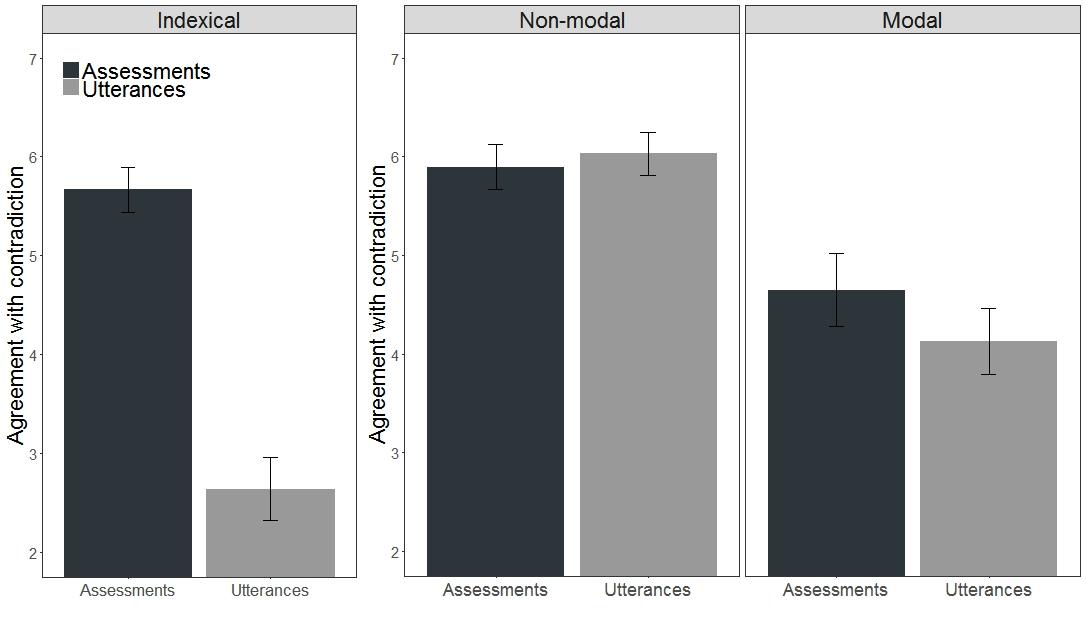
\includegraphics[width=5.5in]{fig2.jpg}\label{fig2}\\
{\bf Figure 2}: Participants' mean level of agreement that at least one of the inspectors' claims must be false. Errors bars indicate $+/- 1 SE$. \\
\end{center}

\noindent Focus first on the {\bf Modal}/{\bf Non-Modal} conditions. We analyzed participants' compatibility judgments in the Modal and Non-modal conditions with a 2 (Claim: Modal vs. Non-modal) x 2 (Case: Utterances vs. Assessments) ANOVA. We found that participants' ratings were significantly affected by whether or not the claims involved an epistemic modal, $F(1,140) = 29.204$, $p < .001$, $\eta_p^2 = .171$, such that they strongly agreed that one of the inspector's claims must be false when they uttered/assessed a non-modal claim ($M = 5.96$, $SD = 1.33$), but not when they uttered/assessed a modal claim ($M = 4.38$, $SD = 2.10$), $t(119.89) = 5.11$, $p < .001$, $d = .902$. By contrast, we did not observe a significant effect of whether the Inspectors made conflicting utterances or conflicting assessments, $F < 0.5$, and most importantly did not find an interaction effect between these two variables, $F < 1.5$, meaning that the \textit{difference} between the modal and non-modal claims did not significantly differ between the {\bf Assessments} and {\bf Utterances} conditions.

Thus, in line with contextualism, but not relativism, participants were more inclined to judge that the two modal (vs non-modal) claims were compatible in the {\bf Utterances} condition.\footnote{This result builds on the recent findings of \cite{katz:2017} who explored a different variant of compatibility judgments about two  utterances across a variety of cases. In the case most similar to ours (the FBI case), they found that about 50\% of participants agreed that the two modal utterances could both be true (at the same time). In addition, they also included two ``screening'' questions which involved the compatibility of two conflicting utterances of a non-modal or indexical claim. Further complementing the patterns we observed, only 24\% of participants judged that both non-modal utterances could be true, while 97\% judged that both indexical utterances could be true. The convergence of these two data sets paints a clear picture of the pattern of judgments about conflicting utterances.} At the same time, in conflict with \textit{both} relativism and contextualism, participants were also more inclined to judge that the two assessments were compatible when they concerned a modal (vs non-modal) claim in the {\bf Assessments} condition. Thus, the above results present a challenge to both contextualist and relativist theories. Before we turn to present our  alternative to orthodox contextualism and relativism, we pause here to discuss a move that may be made on behalf of each theory to account for our data.
%Should we change the polarity here to "less agree that the claims were incompatible"? Technically, we tested incompatibility, not compatibility... 

\subsubsection{Defending orthodox contextualism?}

A contextualist may be tempted to deny {\sc Says-Talk} in order to account for the data in the {\bf Assessments} case. In particular, a contextualist might instead hold that \ul What X said\ur has two interpretations: on one, it refers to the proposition X asserted, while on the other it refers (in context $c$) to the proposition that the sentence X uttered would have expressed had that sentence been uttered in $c$.\footnote{This idea is proposed by \cite{bjornsson:2010} (p. 21) in the course of defending metaethical contextualism.} Given this assumption, in the {\bf Modal Assessments} case, there would be an interpretation of A's utterance of ``What the Chief said is true'' in which it expressed the proposition that the Chief's sentence would have expressed had it been uttered in A's context---namely, that it is possible, given A's evidence that Fat Tony died at the docks. And likewise there would be an interpretation of B's utterance of ``What the Chief said is false'' in which he says that it is not possible given B's evidence that Fat Tony died at the docks. These two propositions are not (necessarily) incompatible. Thus, given this assumption about \ul What X said\urn, the contextualist would be able to predict our results for the {\bf Assessments} conditions.  

The trouble with this assumption is that it does not sit well with the pattern of results from the \textbf{Indexical} conditions, which are correctly predicted by {\sc Says-Talk}. Consider the results from the {\bf Indexical Assessments} case, where the two Inspectors made conflicting assessments about the Chief's utterance of ``I have served on the police force for twenty years.'' In this case, participants strongly agreed that at least one of the Inspectors claims must be false ($M = 5.67$, $SD = 1.40$), and agreed much more strongly than in the \textbf{Indexical Utterances} case, ($M = 2.64$, $SD = 1.96$), $t(68.69) = -7.82$, $p < .001$, $d = 1.77$ (see Fig. 2). In this \textbf{Indexical Assessements} case, {\sc Says-Talk} predicts that ``What the Chief'' said refers to the proposition that the Chief has served on the police force for twenty years. A says of this proposition that it is true, while B says of this proposition that it is false. Since at least one of these claims must be false, {\sc Says-Talk} correctly predicts strong agreement with (Q). By contrast, if the contextualist response above is correct, we expect there to be an interpretation of A's/B's utterances of ``What the Chief said is true''/``What the Chief said is false'' in which A says that A has served on the police force for more than twenty years and B says that B has not served on the police force for more than twenty years. But these two claims are clearly compatible.\footnote{This interpretation of our data is bolstered by participants' responses to a check question which asked them who the Inspectors were talking about when they spoke. In the \textbf{Indexical Utterances} condition, participants overwhelmingly thought Inspector A and Inspector B had themselves in mind ($79.49\%$ and $82.05\%$, respectively). In the \textbf{Indexical Assessments} condition, participants instead overwhelmingly thought Inspector A and Inspector B had the Chief in mind ($84.62\%$ in both cases).} We take these data to both confirm {\sc Says-Talk} and cast doubt on this kind of response on behalf of the contextualist.

\subsubsection{Defending orthodox relativism?}

A relativist may be tempted to reject both {\sc Says-Talk} and {\sc Deflationism} to account for our data. On this kind of approach, expressions like \ul What X said\urn/\ul X's claim\ur refer to something that encodes both the proposition X asserted and the context in which it was asserted: perhaps the act of X's assertion. We'll model this as a pair of a proposition (the content of the assertion) and a context (the context of the assertion): $\langle p,c\rangle$. This approach then adopts an ambiguity view of ``is true''/``is false.'' For example, focus on falsity. On one interpretation ``is false'' is deflationary; it maps an assertion to the negation of its content. On that interpretation, \ul What X said is false\ur is equivalent to the negation of the proposition X asserted. On the other interpretation, ``is false'' means ``false-as-uttered'': an assertion $\langle p,c\rangle$ is true-/false-as-uttered iff $p$ is true/false at $c$. Importantly, then, an assertion $\langle \lozenge p, c\rangle$ is true-/false-as-uttered iff $\lozenge p$ is true/false relative to evidence $f_c$. 

To see how this can predict the data from $\S$\ref{2.3}, first consider the {\bf Modal Utterances} case, where A says, ``Fat Tony could have died at the docks'' and B says, ``Fat Tony couldn't have died at the docks'' (in different contexts). If participants understand ``is false'' in (Q) as deflationary, they will agree with it---this is because they should think that either Fat Tony could have died at the docks or Fat Tony couldn't have died at the docks. But if participants understand ``is false'' in (Q) as false-as-uttered, they should disagree with this statement, as long as they think that (i) the evidence in A's context is compatible with Fat Tony having died at the docks and (ii) the evidence in B's context is not compatible with Fat Tony having died at the docks. In this case, both A's and B's assertions would be true-as-uttered.  
%A's assertion was $\langle \lozenge d, c_A\rangle$, and B's assertion was $\langle \lnot\lozenge d, c_B\rangle$. If participants understand ``is false'' in (Q) as deflationary, they should agree with it, since (relative to the information in their context) either $\lozenge d$ is false or $\lnot\lozenge d$ is false. But if participants understand ``is false'' in (Q) as false-as-uttered, they should disagree with this statement, as long as they think that (i) the evidence in A's context is compatible with Fat Tony having died at the docks and (ii) the evidence in B's context is not compatible with Fat Tony having died at the docks. In this case, both A's and B's assertions would be true-as-uttered. 

Next, turn to the {\bf Modal Assessments} case. If participants understand Inspector A's utterance of ``What the Chief said is true,'' Inspector B's utterance of ``What the Chief said is false,'' and the statement ``At least one of the Inspectors' claims must be false'' all in the deflationary way, then they should agree with the latter statement. This is because on this interpretation A asserts that Fat Tony could have died at the docks, B asserts the negation of this proposition, and one of these two propositions must be false. However, if instead they understand ``At least one of the Inspectors' claims must be false'' as false-as-uttered, they should disagree with this statement, at least if they think that (i) A's evidence is compatible with Fat Tony having died at the docks and (ii) B's evidence is not compatible with Fat Tony having died at the docks. For then, both A's and B's assertions would be true-as-uttered.

One challenge to this strategy is that, if ``true'' and ``false'' are genuinely ambiguous in the proposed way, it seems that it should be possible to disambiguate them in such a way to make sense of C's response in the following dialogue:

\ex.[A:] Fat Tony might be dead.

\ex.[B:] What A said is false.

\ex.[C:] {\#}I agree with you B---what A said is false; but also, A's claim is true since A didn't have the evidence proving Fat Tony is alive.  

Yet, to our ears, such dialogues sound irreparably incoherent (cf. \cite{macfarlane:2009}: 248). Compare this dialogue with one involving a polysemous term, such as ``book,'', which may mean either ``a bound collection of pages'' or ``a literary work'':

\ex.[D:] (pointing to a bound volume with blank pages) This is a book.

\ex.[E:] I agree with you D---that is a book; but it also isn't a book since it's not a literary work.

In contrast with with the exchange between B and C, E's response to D here seems coherent. Thus, we think that the relativist strategy of appealing to an ambiguity in ``is true''/``is false'' will face some steep challenges.

%A second challenge is that there is some reason to think that \ul What X said is true\ur does not involve predicating ``is true'' of X's assertion, but rather of the content of X's claim. Although we say things like \ul X's assertion was true\urn, it is quite odd to say \ul X's act of assertion was true\urn. This is some reason to think that the former expression really targets the content of X's assertion, not X's assertion itself, and that ``is true''/``is false'' in ordinary English are not predicates of assertions, but only of contents (cf. \cite{macfarlane:2005a}: 322-323; \cite{macfarlane:2008b}: 93-94).\footnote{We might drop the idea that \ul What X said\ur refers to X's assertion and just hold that it refers to something that is representable formally as a context, content pair. This would allow the theory to work formally, at the expense of making it somewhat mysterious. Furthermore, we might wonder if there are other expressions which would unambiguously refer to the content of an assertion. If there are, we could test this theory by running our experiments using this expression, to see if the results differ from the results we found with \ul What X said\urn.}  

%Next, we consider a response to our data on behalf of the orthodox relativist. The orthodox relativist may be tempted to respond that \ul might p\ur has an interpretation on which it contains a covert ``for all I know'' (FAK) operator in its logical form (cf. \citealt{macfarlane:2014a}: 274-275). Then there would be an interpretation of \ul might p\ur that is equivalent to \ul for all I know, might p\urn. The possibility of this interpretation would allow the orthodox relativist to predict the data in the {\bf Modal Utterances} case (in the same way that the contextualist does). To account for the data in the {\bf Modal Assessments} case, the relativist might opt to deny {\sc Deflationism} and opt for a contextualist theory of truth. We will focus on the first move here, since we will come back to the latter move below in $\S$\ref{3}. Our worry with positing covert FAK operators is that, if it is possible to add a covert FAK operator in the logical form of \ul might p\urn, we expect to be able to do so in non-modal sentences as well. But then we expect that in the {\bf Non-Modal Utterances} case, there should be a reading of A's claim which would be equivalent to, ``For all A knows, Fat Tony died at the docks,'' and there should also be a reading of B's claim which would be equivalent to, ``For all B knows, Fat Tony did not die at the docks.'' Since these two claims are compatible,  we should then predict that participants would agree with (Q) at roughly the same rate across the {\bf Modal} and {\bf Non-Modal Utterances} case. But we found instead that participants more strongly agreed with (Q) in {\bf Non-Modal Utterances} than in {\bf Modal Utterances}. So we think our data casts doubt on this kind of response by the orthodox relativist.

We conclude that our data raise a challenge to both orthodox contextualist and orthodox relativist theories. We turn next to a different approach to thinking about modal semantics that we think is independently plausible and can account for the data discussed in this section.

\section{Contextualist Situation Semantics}
\label{3}

In this section, we offer a new theory of epistemic modals, and show how it can predict the complete pattern of judgments we found. As a brief preview: our theory will accept context-dependence (C1), and truth relativism (R2), and deny {\sc Deflationism} in favor of a contextualist theory of truth. 

We state our theory within a situation semantic framework, on which propositions are sets of situations rather than sets of worlds (cf. \citealt{kratzer:1989, kratzer:2012}).\footnote{A centered worlds framework would have worked just as well for our purposes (cf. \citealt{egan:2007}).} A situation is a possibly partial world---that is, each situation determines a unique world, but there may be distinct situations which determine the same possible world. A proposition $p$ is true at situation $s$ iff $s\in p$. Since it is possible for some proposition $p$ to be true at some situations at some world but not others at that same world, adopting a situation semantic framework allows us to predict truth-relativism, (R2). 

We capture context-dependence, (C1), by allowing that the same epistemic modal sentence may vary in what proposition it expresses at different contexts of utterance. Just as with orthodox contextualist theories, we hold that epistemic modal sentences are about particular modal bases. However, unlike orthodox contextualist theories, we hold that some epistemic modal claims are about modal bases that may vary in output across situations; hence, on our theory, a modal base is now a function from a situation (rather than a world) to a set of worlds. This will allow us to define modal bases which are {\it situation-variant}: such modal bases vary in output across situations that share the same world. We can also define {\it situation-invariant} modal bases: these vary in output only across situations at different worlds. To see the difference here, consider the following two epistemic modal bases:

\begin{itemize}
\item X's evidence at $t$.
\item The best available evidence.
\end{itemize}

\noindent X's evidence at $t$ is situation-\textit{invariant}: it varies across worlds (insofar as it X could have had different information than X in fact had) but not across situations at the same world. By contrast, the best available evidence is arguably situation-\textit{variant}, since different evidence is available in different situations.\footnote{Some independent evidence that epistemic modal claims can be interpreted as about situation-variant modal bases or situation-invariant modal bases comes from data about retraction. Whether you should retract a claim depends on whether it is true in your situation. If you utter \ul might p\ur in a context in which it is assigned a situation-variant modal base, and you later learn $\lnot p$, then you should retract your utterance in light of this new evidence, since your claim would now be false at your new situation. Suppose instead you utter \ul might p\ur in a context in which it is assigned a situation-invariant modal base (about, say, your current evidence), and your current evidence is compatible with $p$. Then if you later learn $\lnot p$, you would not be required to retract your previous utterance, since it would still be true at your new situation. The observation (from \citealt{fintelgillies:2011}) that there are two possible responses (retract, or stick to one's guns) after uttering \ul might p\ur and later learning $\lnot p$ is thus prima facie evidence that we sometimes use epistemic modal sentences to express situation-variant and sometimes situation-invariant claims:

\begin{itemize}
\item[] A:  The keys might be in the drawer. 
\item[] B:  No, I have them with me. Why did you say that? 
	\bitem
	\item A1:  Oh, I guess I was wrong. 
	\item A2:  I didn't say they were in the drawer, only that they might be, and they might have been! 
	\eitem 
\end{itemize}

}
%\noindent Here, (A1)'s response indicates that she had intended the situation-variant interpretation of her modal claim: one whose truth value changes as she learns more information. By contrast, (A2)'s response indicates that she had intended the situation-invariant interpretation of her modal claim, and that it was centered on the information she had when uttering it.}

We continue to accept {\sc Says-Talk}. Finally, we reject {\sc Deflationism} in favor of {\sc Contextualist Truth/Falsity}:

\ex.[] {\sc Contextualist Truth/Falsity}\\	
	{The proposition expressed by \ul What X said is true\ur (\ul What X said is false\urn) is equivalent to the proposition that the referent of \ul What X said\ur is true (false) at the situation of $c$.} 

{\sc Contextualist Truth/Falsity} predicts that a truth/falsity-assessment of $p$ is a claim that $p$ is true at the situation in which the claim is being made. Suppose that $p$ is the proposition expressed by Z's utterance, and that $p$ is in fact true at $s_1$ and false at $s_2$. Suppose X says, ``What Z said is true'' in situation $s_1$ and Y says, ``What Z said is false'' in situation $s_2$. Then, we predict that both X and Y's claims are true. As we will see in a moment, this will be the key to predicting the data we found in the {\bf Modal Assessments} case.\footnote{A potential worry is that {\sc Contextualist Truth/Falsity} predicts that truth-/falsity-ascriptions are either necessarily true or necessarily false. One way to avoid this problem and still hold that truth-/falsity-ascriptions convey information about particular situations is to appeal to counterpart relations among situations. Thus, instead of indexing ``true'' and ``false'' to a particular situation, we rather index them to a function from situations to situations, $g_s$, that is anchored to a particular situation, $s$. The idea is that $g_s$ maps a situation $s'$ to the counterpart of $s$ that is world-mates with $s'$. Then, the view is that \ul What X said is true\ur expresses the proposition (at $c$) that the proposition referred to by \ul What X said\ur at $c$ is true at the counterpart of $s_c$; i.e., the proposition $\{s: p_X$ is true at $g_{s_c}(s)\}$ (where $p_X$ is the proposition that X asserted).}  

\subsection{Predicting the Data}
\label{3.1}

Recall the {\bf Modal Utterances} case, where Inspector A looks at the evidence at the docks and utters, 

\ex. Fat Tony could have died at the docks. \label{ft1}

while Inspector B sees Fat Tony plant the evidence and utters,

\ex. Fat Tony could not have died at the docks. 

We aim to predict the possibility of semantically competent people disagreeing about (Q) in this scenario:

\ex.[(Q)] At least one of Inspector A or Inspector B's claims must be false.

We predict this by allowing that there are two interpretations of A and B's claims. On one interpretation, Inspector A made a claim about what was possible given what he knows from the evidence at the docks (let $d$ be the proposition that Fat Tony died at the docks):

\ex.[] $\{s: \exists w\in f_{\it docks}(s): w\in d\}$. 
%$: the evidence from the docks at $t,w_s$ is not compatible with $d\}$. 

Similarly, perhaps Inspector B made a claim about what was possible given what he knows from the security camera footage:

\ex.[] $\{s: \lnot\exists w\in f_{\it camera}(s): w\in d\}$ 
%$: the evidence from the security camera at $t,w_s$ is not compatible with $d\}$. 

It's not hard to imagine a continuation of the story that (tacitly) supports this interpretation of the inspectors' claims. For example, the Chief might commend both Inspectors on their conclusions: Inspector A because he correctly assessed which possibilities had been left open by what he learned at the docks, and Inspector B because he correctly assessed which possibilities had been left open by what he learned from the security camera. On this intuitive picture, there is no reason that one of the Inspectors' claims must be false, so someone interpreting the case this way should think that (Q) is false.

But this is only one possible way of interpreting the two inspectors' claims. A different interpretation is that both Inspector A and Inspector B made claims about the best available evidence in the case. On this interpretation, Inspector A asserted the following proposition, while Inspector B asserted its negation (where $f_{\it best}$ is situation-variant):

\ex.[] $\{s: \exists w\in f_{\it best}(s): w\in d\}$
%$\{s$: the best available evidence in $s$ is compatible with $d\}$.

On this interpretation, relative to any situation, at least one of A and B's claims must be false. Thus, someone interpreting the Inspectors this way should think that (Q) is true. Variability in whether the modal base is situation-variant or situation-invariant is how our contextualist situation semantics allows for agreement and also disagreement with (Q) in the {\bf Modal Utterances} case, and thus allows us to predict the mid-point agreement observed on average. 

Turn next to the {\bf Modal Assessments} case. In this case, the Chief utters \ref{ft1}; Inspectors A and B (with the same evidence as above, and in different contexts from the Chief and each other) overhear the Chief's utterance and say, respectively: 

\ex. What the Chief said is true. 

\ex. What the Chief said is false. 

In this case, there is a unique proposition expressed by the Chief; what our theory predicts about (Q) depends on what proposition this is. One possibility is that the Chief intended to make a claim just about what he knows at the time. Perhaps he wanted to state something he could be very confident was true, and to which he could remain committed even after he gained further evidence. On this interpretation, the Chief asserted the content (where $f_{\it Chief}$ is situation-invariant):

\ex.[] $\{s: \exists w\in f_{\it Chief}(s): w\in d\}$
%$\{s:$ the Chief?s evidence at $t,w_s$ is compatible with $d\}$.

Then, by {\sc Contextualist Truth/Falsity}, Inspector A says that this proposition is true at A's situation, and Inspector B says that this proposition is false at B's situation. But since A's situation and B's situation are at the same world, then the Chief's proposition cannot be true at A's situation and false at B's situation. Therefore, on this interpretation, we predict that (Q) is true: someone interpreting the Chief in this way should thus agree with (Q). 

However, there is another possibility: perhaps the Chief wanted to make a claim about the case overall, a claim which he may have to revise upon learning more information later. That is, on this interpretation Chief instead expressed situation-variant content about the best available evidence:

\ex.[]  $\{s: \exists w\in f_{\it best}(s): w\in d\}$
%$\{s:$ the best available evidence at $s$ is compatible with $d\}$.

Then, by {\sc Contextualist Truth/Falsity}, Inspector A says that this proposition is true at A's situation, and Inspector B says that this proposition is false at B's situation. Given the plausible assumption that in A's situation the best available evidence {\it is} compatible with $d$, then A's claim would be true. And given the equally plausible assumption that at B's situation the best available evidence is {\it not} compatible with $d$, then B's claim would also be true. Therefore, on this interpretation, we predict that (Q) is false: someone interpreting the Chief in this way should thus disagree with (Q).\footnote{An anonymous reviewer suggests that, even in this case, it would be natural for A to retract her claim upon accepting B's claim. If so, this is not immediately predicted by our view. Our theory predicts that A says that the best evidence available in A's situation does not rule out the possibility that Fat Tony died at the docks, which is true even at a situation in which the best available evidence rules out that Fat Tony died at the docks. Still, there may be other reasons why it would be appropriate for A to retract her claim in such a case. Claiming that $p$ is compatible with the best available evidence in a particular situation may implicate that no nearby situation has better available evidence. If so, then learning that the evidence in some nearby situation rules out $p$ would naturally introduce pressure to retract the original claim. We are not convinced that this is the best way to go, but it is worth pointing out that such a case would raise a quite general challenge. There are two intuitions in tension in this kind of case: one is that A and B's claims are incompatible (in our technical sense) and the other is that it would be appropriate for A to retract her claim in light of accepting B's claim (see \cite{yalcinknobe:2014}'s Experiment 4 for a similar case). We hope further work will be done to explore these intuitions empirically.} Taken together, these two interpretive possibilities again allow our theory to predict the midpoint agreement we observed in the \textbf{Modal Assessments} cases.

Finally, we note here why our contextualist situation semantic theory predicts that (Q) is true for the {\bf Indexical Assessments} version of the case. We assume that the semantic value of an indexical like ``I'' is not situation-variant. One strategy is that ``I'' is directly referential and context-sensitive (a la \cite{kaplan:1989}). Then, when the Chief says, ``I have served on the force for more than twenty years,'' she expresses the proposition (let `Chief' be a name that rigidly designates the Chief):%\footnote{Here, we assume that the extension of tense is also not situation-variant. But nothing turns on this point, since by hypothesis A and B's utterances take place at the same time.}

%JSP: Given the space constrints, I thought we should leave this footnote out, since I don't think it's too likely readers will be worried about this, and if they some are, they're also likely to realize it isn't a problem in this case. What do you think?

\ex.[] $\{s$: Chief served on the force for more than twenty years at $w_s\}$. 

When A says, ``What the Chief says is true,'' he asserts that this proposition is true at his situation and when B says,  ``What the Chief says is false,'' he asserts that the negation of this proposition is true at his situation. But since A and B's situations share the same world, at least one of their claims must be false. Thus, we predict the high agreement with (Q) in the {\bf Indexical Assessments} case.

\section{Conclusion}

We argued for evaluating theories of epistemic modals by exploring inter-contextual (in)compatibility judgments. Implementing this strategy, we found a pattern of ordinary judgments that is not predicted by orthodox contextualist or relativist theories. We ended with a novel contextualist situation semantics which {\it does} predict the pattern of judgments we found. 

Stepping back from the particulars of the contextualism/relativism debate over the semantics of epistemic modals, it bears emphasizing that the phenomenon we have uncovered is likely to extend beyond epistemic modal expressions. A much wider range of expressions are known to exhibit some kind of contextual variability (normative expressions, predicates of taste, gradable adjectives, quantifiers, conditionals, and so on), but don't obviously pattern with so-called ``automatic indexicals'', like first person pronouns. A promising possibility is that the present proposal can be fruitfully extended to this wider class of expressions, which have been of central interest across philosophy, linguistics and cognitive science. Critically, the methodology we developed in this paper should be straightforwardly applicable to this wider class of expressions, allowing us to empirically test whether these expressions exhibit the same kind of contextual variation that we have observed in epistemic modals, and to semantically account for this variation where it arises. This extension of the present proposal would not only provide a clearer empirical picture of the context-sensitivity of these expressions themselves, but would shed light on the extent and scope of the underlying phenomenon that gives rise to this kind of pattern in our use of epistemic modals.


\end{doublespace}


\bibliographystyle{authordate1}
\bibliography{Philosophy}
%\bibliography{\string~/Dropbox/Philosophy/bib/Philosophy}


\end{document}